\section{Experiments}
\subsection{Experiment Setup}
For all the experiments, we run the algorithm with one single GPU (NVIDIA Tesla V100) and CPU (Intel Xeon E5-2680). 
Following ~\citet{peng2021amp}, we use the average pose error as the main metric. The average pose error over the whole trajectory of length $T$ with $J$ joints is computed between the pose of the simulated character and the reference motion using the relative positions of each joint with respect to the root joint (in units of meters):
\begin{equation}
\small
    e = \frac{1}{T} \sum_{t\in T} \frac{1}{\lVert J \rVert} \sum_{j \in J} \lVert (p^j_t - p_t^{root}) - (\hat{p}^j_t - \hat{p}_t^{root}) \rVert_2, 
\end{equation}
where $p^j_t$ and $\hat{p}^j_t$ are the position of $j$-th joint of the simulated motion and reference motion at timestamp $t$ in the 3D cartesian space and $root$ refers to the root joint. 
We mainly compare with DeepMimic~\citep{peng2018deepmimic}, Spacetime Bound~\citep{ma2021learning}, and Adversarial Motion Prior (AMP)~\citep{peng2021amp}. Dynamic Time Warping~\citep{sakoe1978dynamic} is applied to synchronize the simulated motion and the reference motion following the convention.

\textbf{Cyclic Motions.} Besides mimicking a single motion clip, a popular benchmark for motion mimicking is to imitate cyclic motions like walking and running, where a single cycle of the motion is provided as the reference motion and the character learns to repeat the motion for 20 seconds. 
Typically, a curriculum is designed to gradually increase the maximum rollout episode to 20 seconds during training~\citep{yang2021efficient, peng2018deepmimic}. In our experiment, we remove all bells and whistles and fix the maximum rollout episode to 4 seconds during the training. DiffMimic can produce a 20-second long cyclic rollout even though it only sees 4-second rollouts in training. {The motion clips are directly borrowed from AMP~\citep{peng2021amp}, which are originally collected from a combination of public mocap libraries, custom recorded mocap clips, and artist-authored keyframe animations.}


\begin{table}[]
    \centering
    \begin{tabular}{cccc}
         \hspace{-10pt}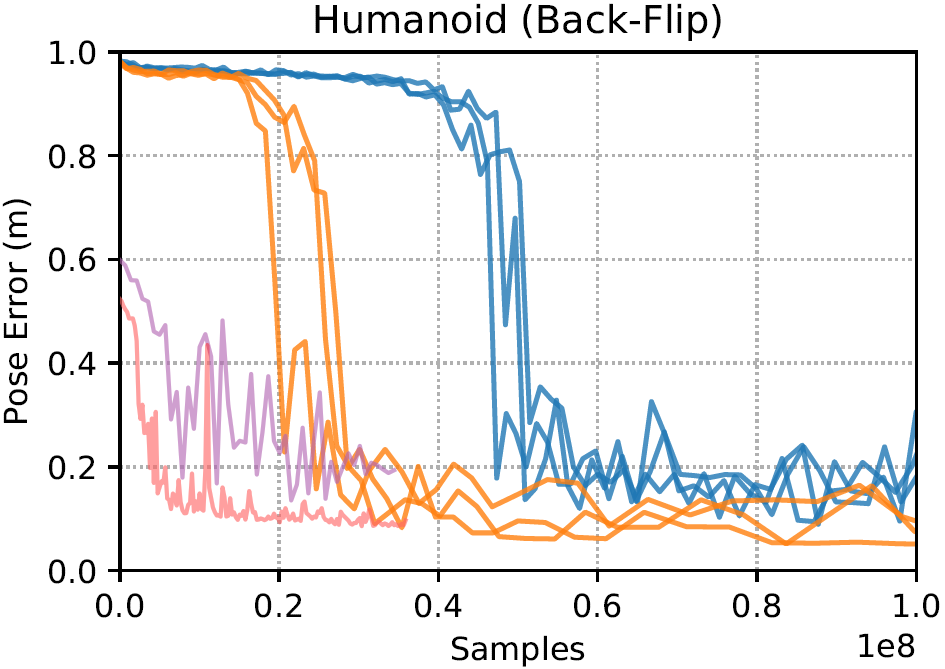
\includegraphics[width=0.23\textwidth]{figures/mixed_backflip.png}
         &
         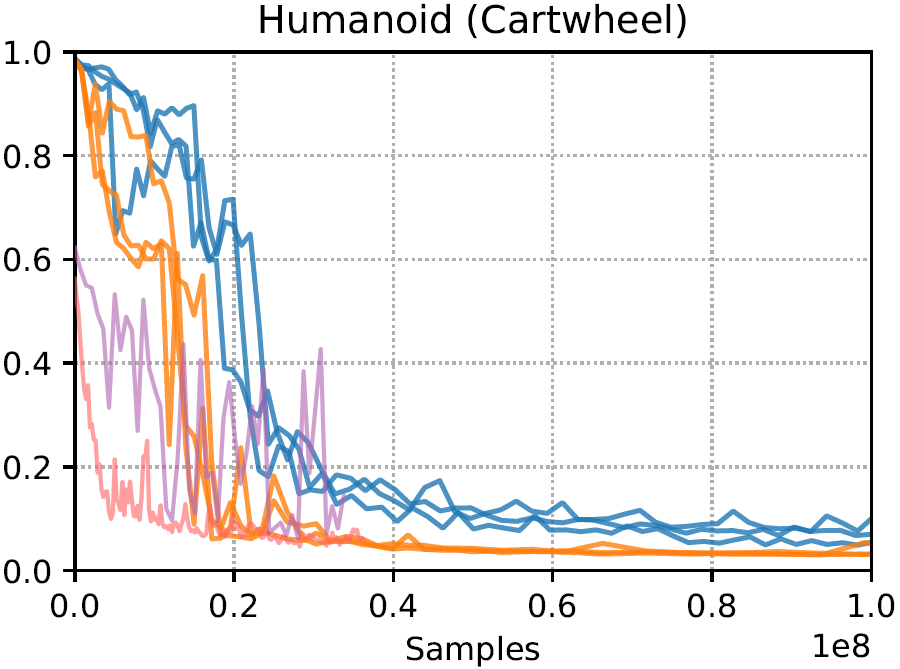
\includegraphics[width=0.23\textwidth]{figures/mixed_cartwheel.png}
         &
         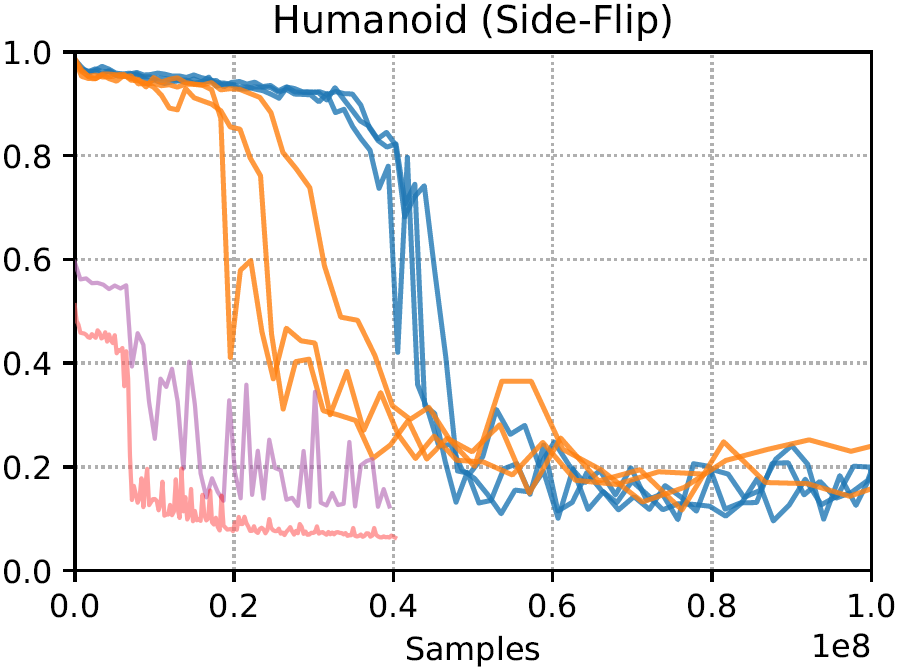
\includegraphics[width=0.23\textwidth]{figures/mixed_sideflip.png}
         &
         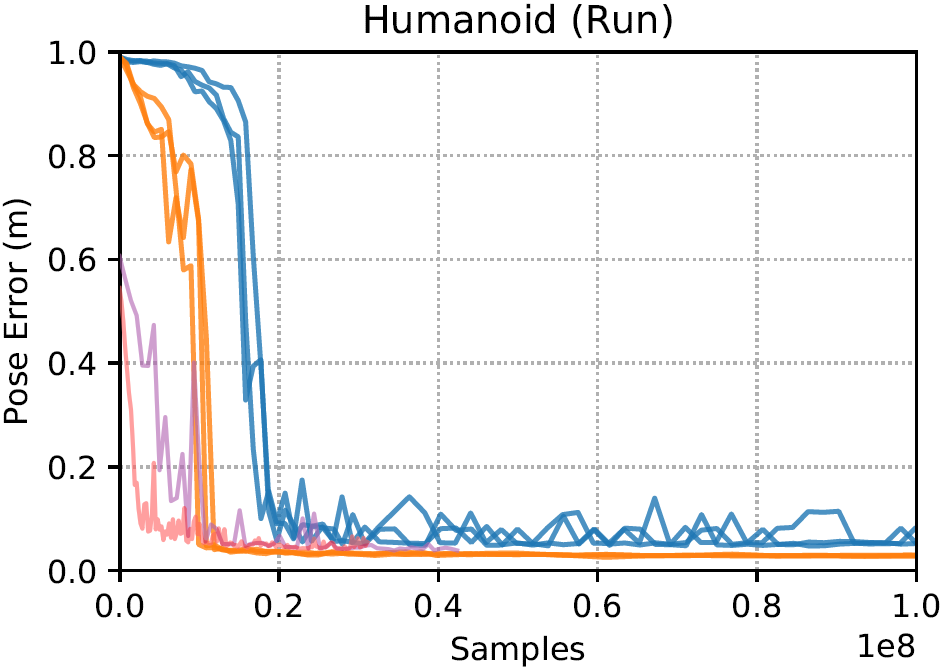
\includegraphics[width=0.23\textwidth]{figures/mixed_run.png}
         \\
         \hspace{-10pt}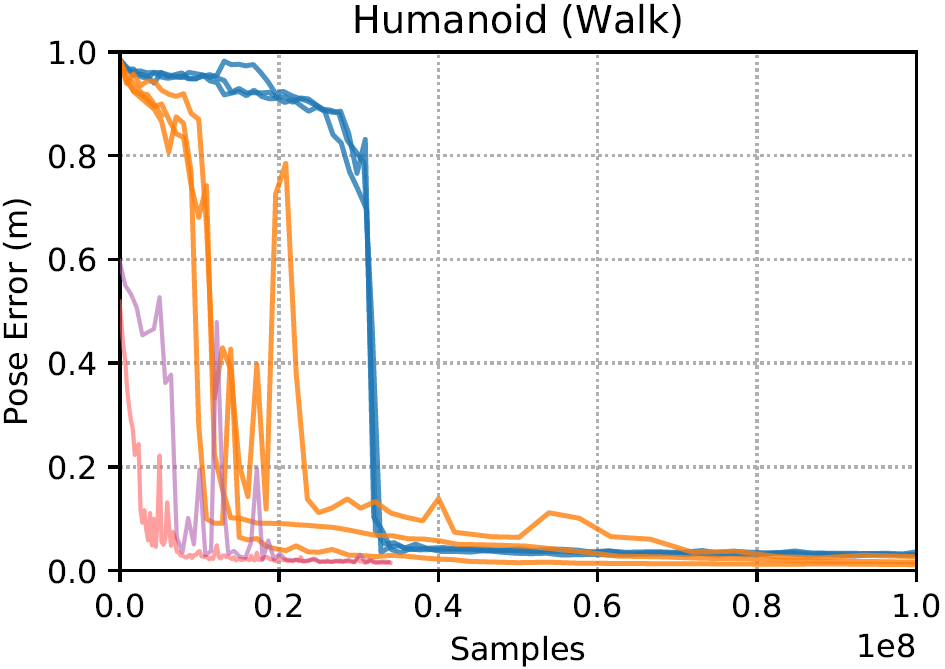
\includegraphics[width=0.23\textwidth]{figures/mixed_walk.png}
         &
         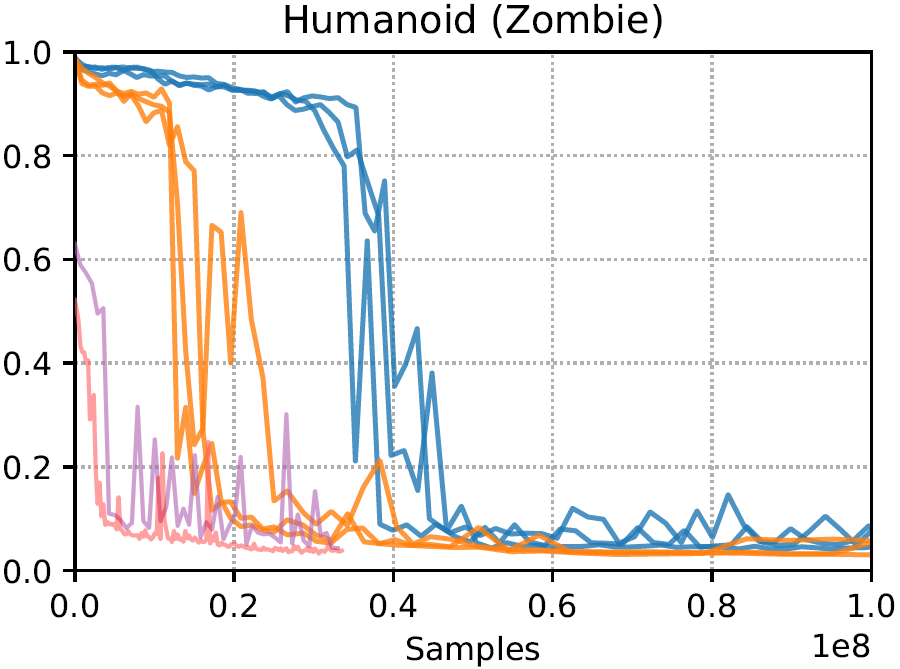
\includegraphics[width=0.23\textwidth]{figures/mixed_zombie.png}
         &
         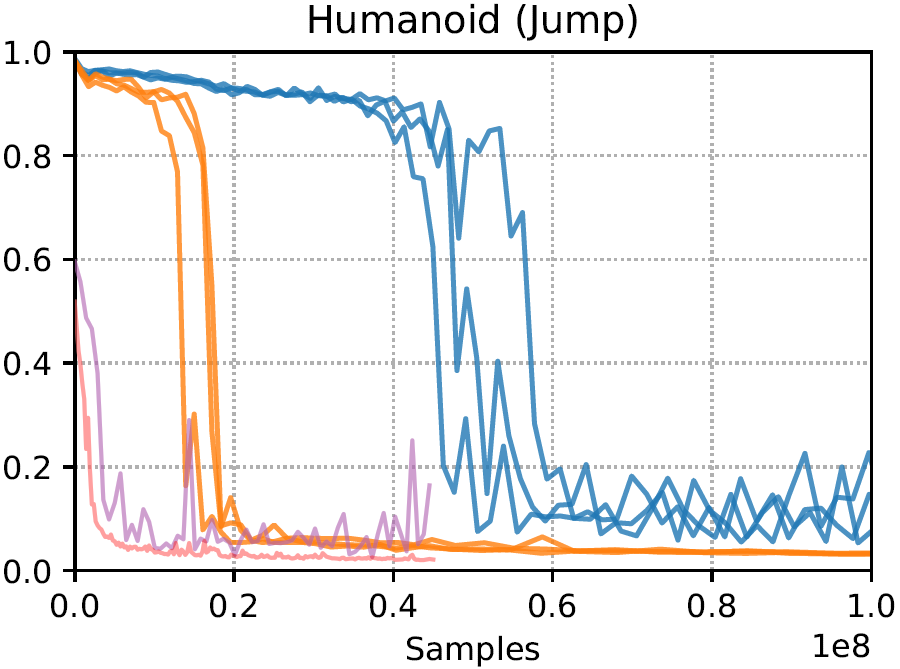
\includegraphics[width=0.23\textwidth]{figures/mixed_jump.png}
         &
         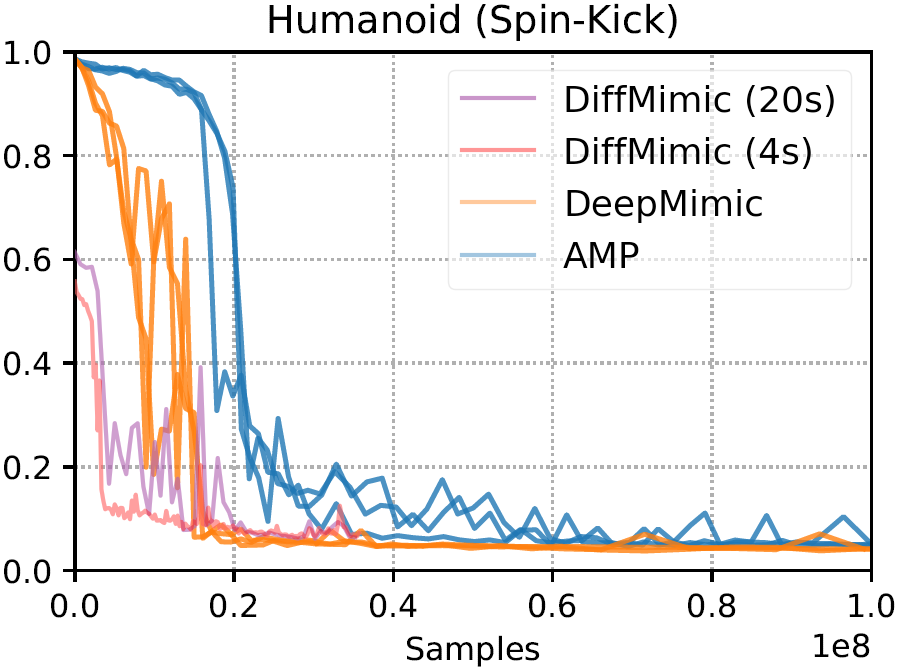
\includegraphics[width=0.23\textwidth]{figures/mixed_spinkick_legend.png}
    \end{tabular}
    \captionof{figure}{Pose error versus the number of samples. DiffMimic (4s): rollout 4 seconds of Diffmimic for evaluation.  DiffMimic (20s): rollout 20 seconds of Diffmimic for evaluation. In general, DiffMimic allows the policy to generate high-quality motions with less than $3.5 \times 10^7$ samples.  
    We refer the readers for more results to the appendix.}
    \label{fig:imitate_one}
\end{table}

\subsection{Comparison on Motion Mimicking}
In this section, we aim to understand 1) efficiency; 2) the quality of the learned policy of DiffMimic. Following the conventions of previous works~\citep{peng2018deepmimic, peng2021amp, ma2021learning}, we count the number of samples required to train the policy to rollout for 20 seconds without falling. The pose error is calculated over the horizon of 20 seconds.

\textbf{Analytical gradients enhance the sample efficiency in motion mimicking.} We show the comparison between DiffMimic, DeepMimic, and Spacetime Bound on sample efficiency in Table~\ref{sampleeff}. DeepMimic is an RL-based algorithm with a careful reward design. Spacetime Bound performs hyperparameter searching for DeepMimic to further enhance the sample efficiency. Our results show that DiffMimic constantly outperforms DeepMimic in terms of sample efficiency. The analytical gradients provided by the differentiable simulation allow us to compute policy gradient with a small number of samples while the RL-based algorithm requires a large batch to have a decent estimate. Compared with Spacetime Bound, DiffMimic is much more stable and consistent over various tasks. We notice that Spacetime Bound may require more samples than DeepMimic even for simple tasks like \textit{Jump}. We show the learning curve of DiffMimic over eight different tasks in Fig.~\ref{fig:imitate_one}. It shows that DiffMimic generally learns high-quality motions (pose error $<$ 0.15) with less than 2e7 samples, even for challenging tasks like \textit{Backflip}. In terms of the wallclock time, DiffMimic learns to perform \textit{Backflip} in 10 minutes and learns to cycle it in 3 hours ($14.88 \times 10^6$ samples), which can be found in our qualitative results.
\begin{wrapfigure}[16]{r}{0.38\columnwidth}
     \centering
     \vspace{-10pt}
         \centering
         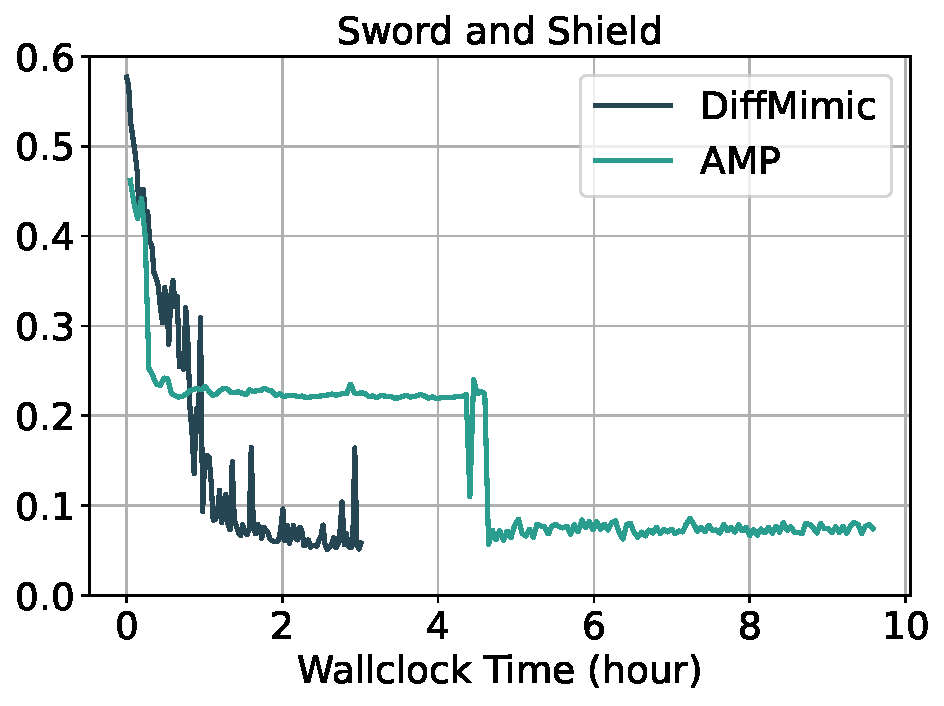
\includegraphics[width=0.38\textwidth]{figures/wallclock_sword.pdf}
     \caption{Wallclock training time versus pose error for DiffMimic and AMP. DiffMimic takes half of the training time required by AMP to have a comparable result.}
    \label{fig:Wallclock time}
\end{wrapfigure}

\textbf{DiffMimic can learn high-quality motions.} The average pose error for 12 different motion tasks is shown in Table~\ref{poseerror}. DiffMimic outperforms AMP consistently and has comparable performance to DeepMimic. 
Noticeably, DiffMimic only needs to see the demonstrations of 4 seconds to achieve a similar performance of DeepMimic with 20 seconds cyclic rollout, which indicates stable and faithful recovery of the reference motion. This further corroborates the efficacy of DiffMimic. 

\textbf{Analytical gradients accelerate the learning speed in motion mimicking.} As it generally takes more time to compute analytical gradients than the estimated one, it is natural to compare the wall-clock time for each algorithm. Since the implementation of DeepMimic does not utilize GPU for parallelization, we choose to compare DiffMimic with AMP. The implementation of AMP utilizes the highly parallelized environment, IsaacGym~\citep{makoviychuk2021isaac}. Both approaches do not require manual reward design and utilize GPU for acceleration. We compare DiffMimic and AMP on a task where a humanoid character is wielding a sword and a shield to perform a 3.2-second attack move (shown in Appendix Fig.~\ref{fig:sword}). The hyperparameter of AMP is from its official release of code.
We show the comparison with respect to wallclock time in Fig.~\ref{fig:Wallclock time}. %
DiffMimic takes half of the training time required by AMP to have a comparable result.



\begin{table}[t]
\caption{Pose error comparison in meters.  $\textrm{T}_\textrm{cycle}$ is the length of the reference motion for a single cycle. The error is averaged on 32 rollout episodes with a maximum length of 20 seconds.}
\fontsize{8.8}{9}\selectfont
\begin{center}
\begin{tabular}{lcccc}
\toprule
Motion & $\textrm{T}_\textrm{cycle}$(s) &  DeepMimic & AMP & Ours\\
\midrule
Back-Flip & 1.75 & 0.076 $\pm$ 0.021 & 0.150 $\pm$ 0.028 & 0.097 $\pm$ 0.001 \\
Cartwheel & 2.72 & 0.039 $\pm$ 0.011 & 0.067 $\pm$ 0.014 & 0.040 $\pm$ 0.007 \\
Crawl & 2.93 & 0.044 $\pm$ 0.001 & 0.049 $\pm$ 0.007 & 0.037 $\pm$ 0.001 \\
Dance & 1.62 & 0.038 $\pm$ 0.001 & 0.055 $\pm$ 0.015 & 0.070 $\pm$ 0.003 \\
Jog & 0.83 & 0.029 $\pm$ 0.001 & 0.056 $\pm$ 0.001 & 0.031 $\pm$ 0.002 \\
Jump & 1.77 & 0.033 $\pm$ 0.001 & 0.083 $\pm$ 0.022 & 0.025 $\pm$ 0.000 \\
Roll & 2.02 & 0.072 $\pm$ 0.018 & 0.088 $\pm$ 0.008 & 0.061 $\pm$ 0.007 \\
Run & 0.80 & 0.028 $\pm$ 0.002 & 0.075 $\pm$ 0.015 & 0.039 $\pm$ 0.000 \\
Side-Flip & 2.44 & 0.191 $\pm$ 0.043 & 0.124 $\pm$ 0.012 & 0.069 $\pm$ 0.001\\
Spin-Kick & 1.28 & 0.042 $\pm$ 0.001 & 0.058 $\pm$ 0.012 & 0.056 $\pm$ 0.000\\
Walk & 1.30 & 0.018 $\pm$ 0.005 & 0.030 $\pm$ 0.001 &  0.017 $\pm$ 0.000 \\
Zombie & 1.68 & 0.049 $\pm$ 0.013 & 0.058 $\pm$ 0.014 & 0.037 $\pm$ 0.002 \\
\bottomrule
\end{tabular}
\label{poseerror}
\end{center}
\end{table}



\begin{table}[t]
\caption{Number of samples required to roll out 20 seconds without falling in $(10^6)$. {Percentage: change in the fraction of the DeepMimic samples.}}
\begin{center}
\begin{tabular}{lcr|r|r}
\toprule
Motion & $\textrm{T}_\textrm{cycle}$(s) &  DeepMimic  & Spacetime Bound  & Ours\\
\midrule
Back-Flip & 1.75 & 31.18 & 41.20 \plusstyle{+32.1\%} & 14.88 \minusstyle{-52.2\%} \\
Cartwheel & 2.72  & 30.45 & 17.35 \minusstyle{-43.0\%} & 13.92 \minusstyle{-54.2\%}\\
Walk & 1.25  & 23.80 & 4.08 \minusstyle{-79.5\%} & 7.92 \minusstyle{-66.7\%} \\
Run & 0.80  & 19.31 & 4.11 \minusstyle{-78.7\%} & 8.16 \minusstyle{-57.7\%} \\
Jump & 1.77  & 25.65 & 41.63 \plusstyle{+77.8\%} & 5.28 \minusstyle{-79.4\%} \\
Dance & 1.62  & 24.59 & 10.00 \minusstyle{-59.3\%} & 16.56 \minusstyle{-32.6\%} \\
\bottomrule
\label{sampleeff}
\end{tabular}
\end{center}
\end{table}



\subsection{Ablation on Truncation length}

Training the policy with DPS would suffer from the vanishing/exploding gradients and local optimal. Recent research~\citep{xu2022accelerated} points out that such a problem can be mitigated by a truncated learning window, which splits the entire trajectory into segments with shorter horizons. we carried out experiments to validate whether such an idea can be directly applied in motion mimicking with DPS. Truncation length refers to the horizon over which the gradient is calculated. The quantitative results are shown in Fig.~\ref{tab:ablation}. Indeed, it is difficult to learn a good policy by propagating the gradient through a whole trajectory that is long. In addition, simply splitting the whole trajectory into segments would worsen the final performance. We hypothesize the naive truncation of the trajectory creates discontinuities in the whole trajectory whereas motions in the trajectory are highly interdependent. For example, how to flip in mid-air closely relates to how the character jumps. We see this as a strong call for a better strategy to handle these two challenges in motion mimicking with DPS.
\subsection{Ablation on Demonstration Replay}

\begin{table}[t]
    \centering
    \vspace{-10pt}
    \begin{tabular}{cccc}
      \hspace{-10pt}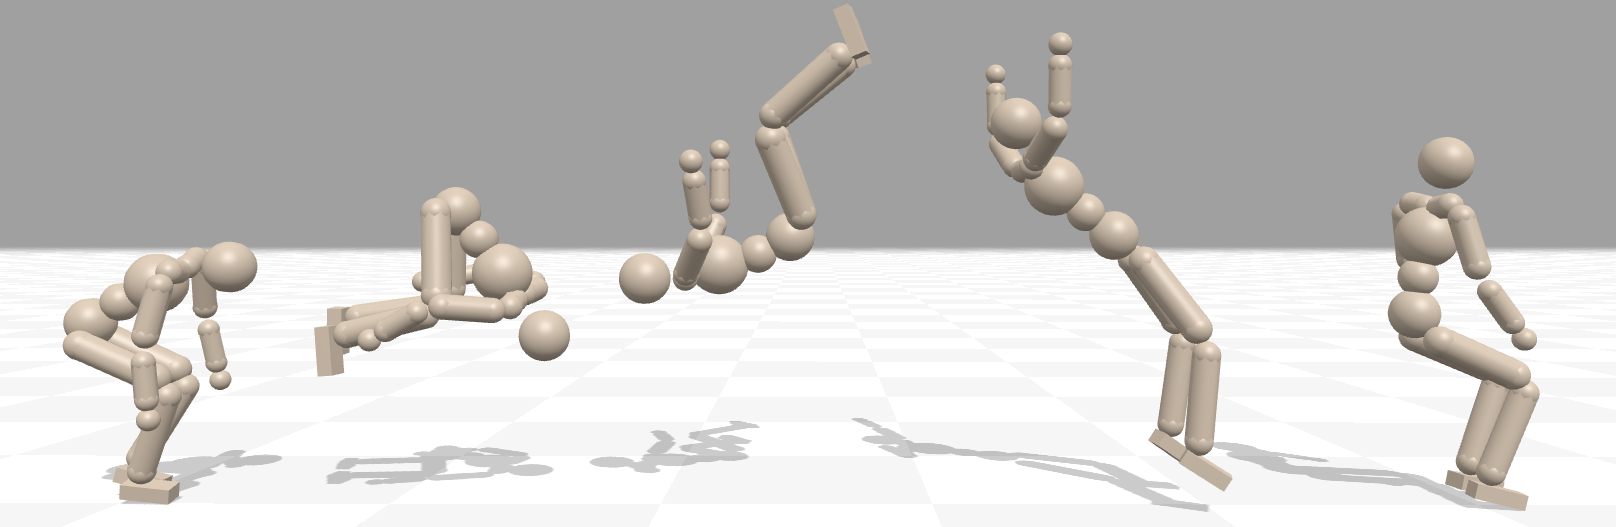
\includegraphics[width=0.4\textwidth]{figures/qp/backflip_demo.png}
      &  
      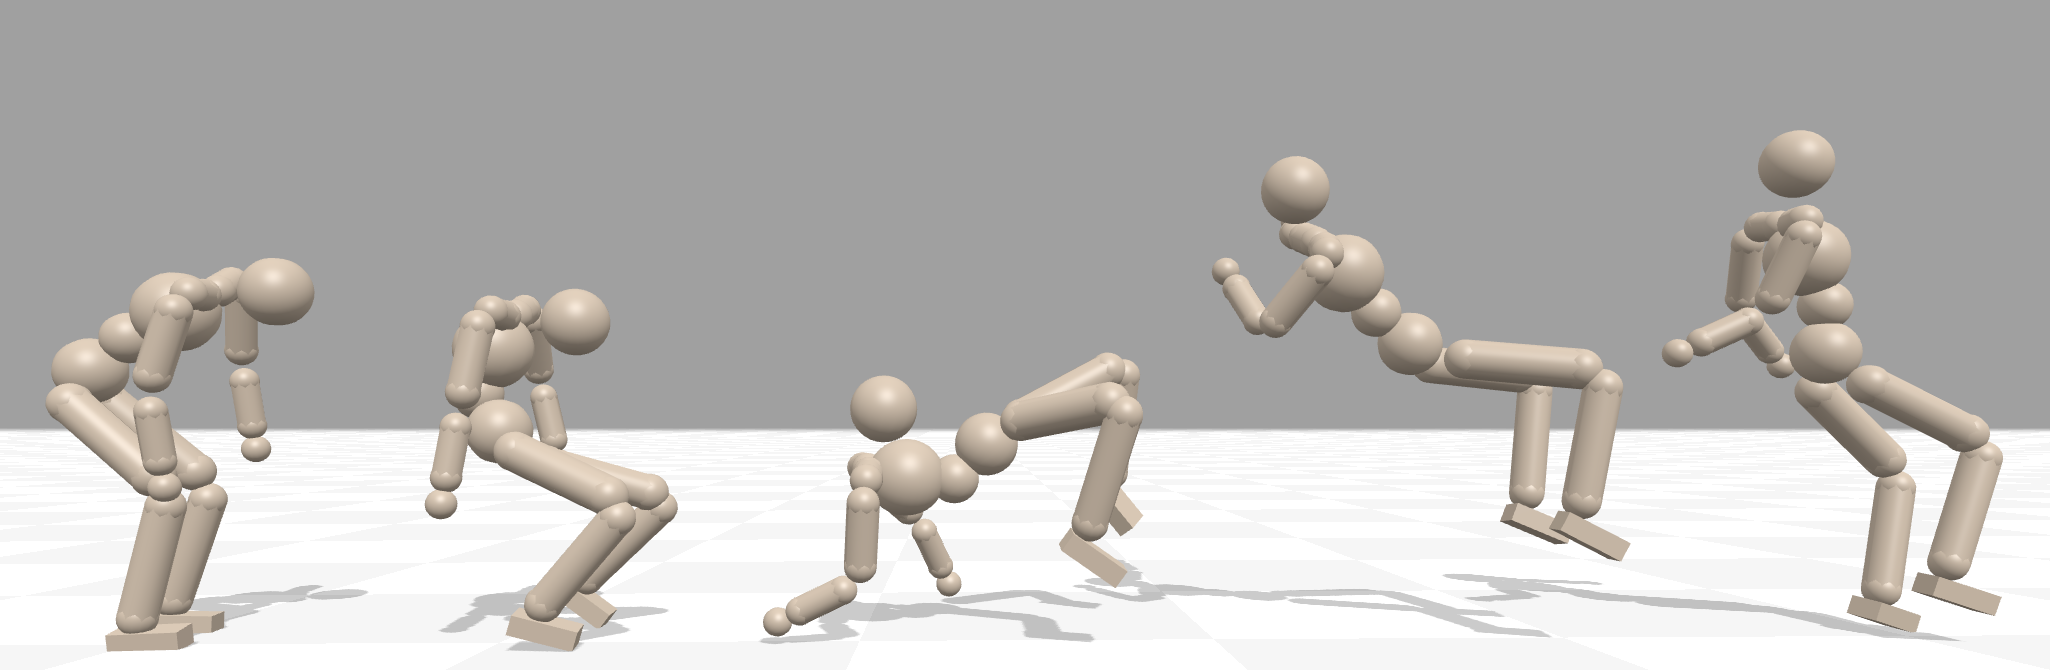
\includegraphics[width=0.4\textwidth]{figures/qp/backflip_trunc1000.png}
        \\
         (a) Reference motion.
         &
         (b) Full Horizon Gradient.
        \\
     \hspace{-10pt}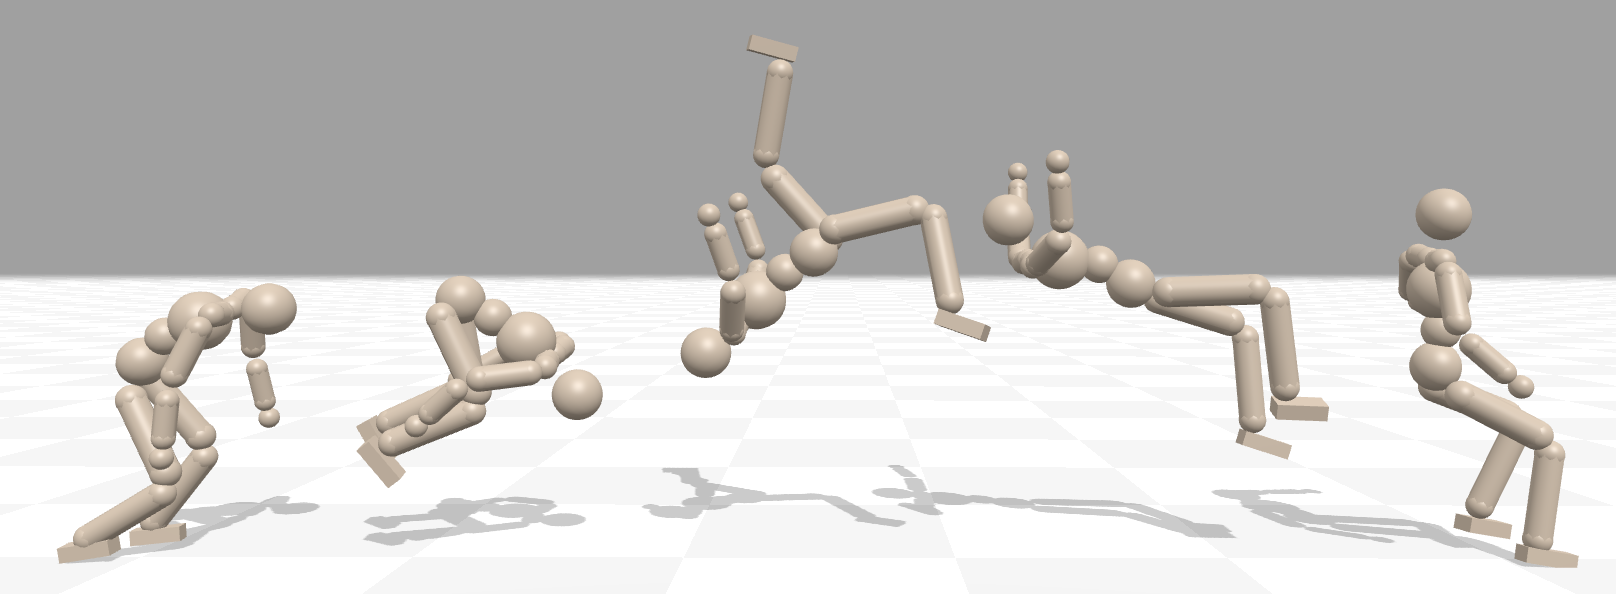
\includegraphics[width=0.4\textwidth]{figures/qp/backflip_random.png}
      &  
      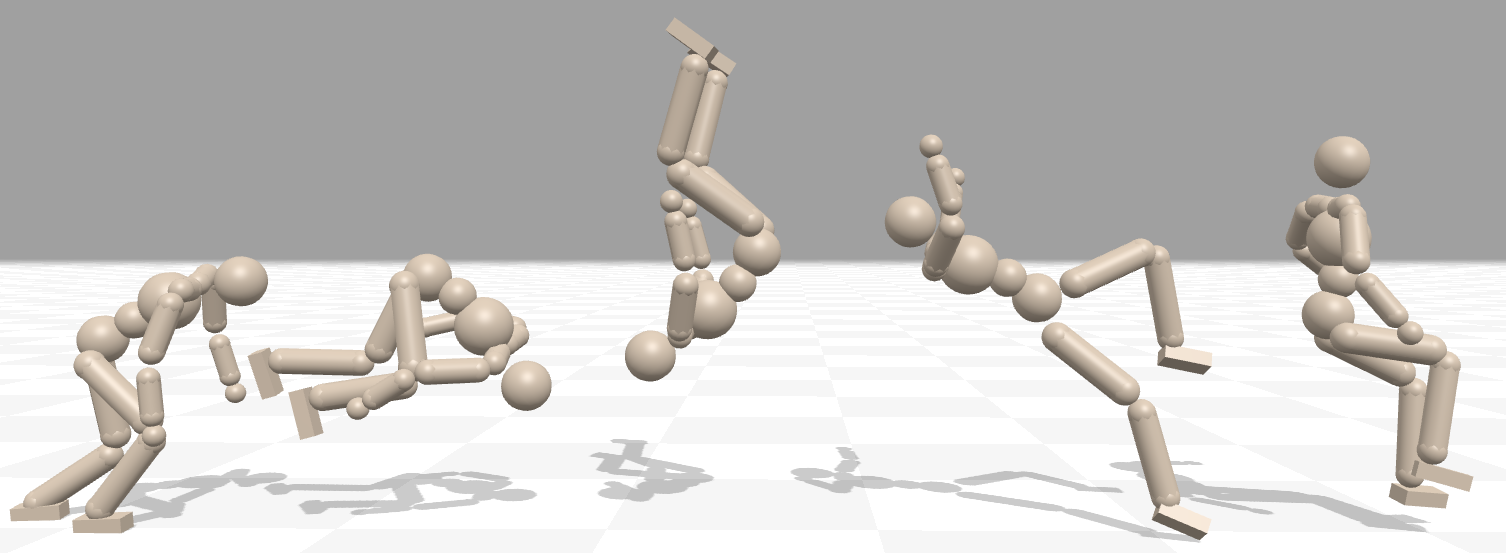
\includegraphics[width=0.4\textwidth]{figures/qp/backflip_err0.4.png}
        \\
        (c) Demonstration Replay (Random).
         &
        (d) Demonstration Replay (Threshold).
    \end{tabular}
    \captionof{figure}{Qualitative results of three variants of DiffMimic with respect to demonstration replay. The policy trained with full horizon gradient fails to jump up. The policy trained with Demonstration Replay (Random) fails to recover the reference motion faithfully. }
    \label{fig:vis_ablation}
\end{table}





\begin{table}[]
    \centering
    \begin{tabular}{ccc}
    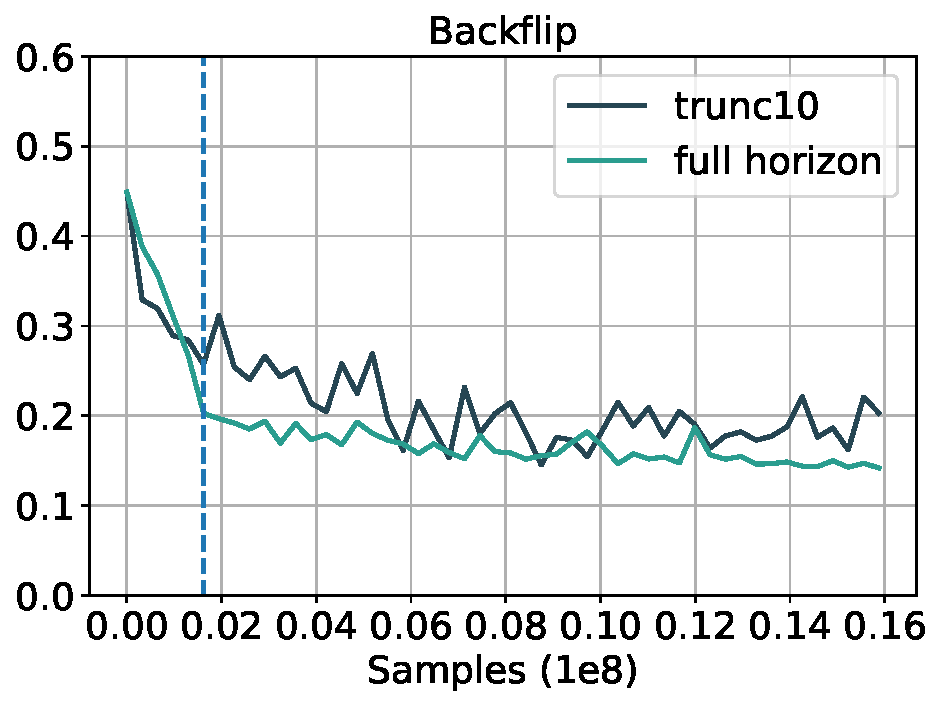
\includegraphics[width=0.3\textwidth]{figures/trunc_backflip.pdf}&
    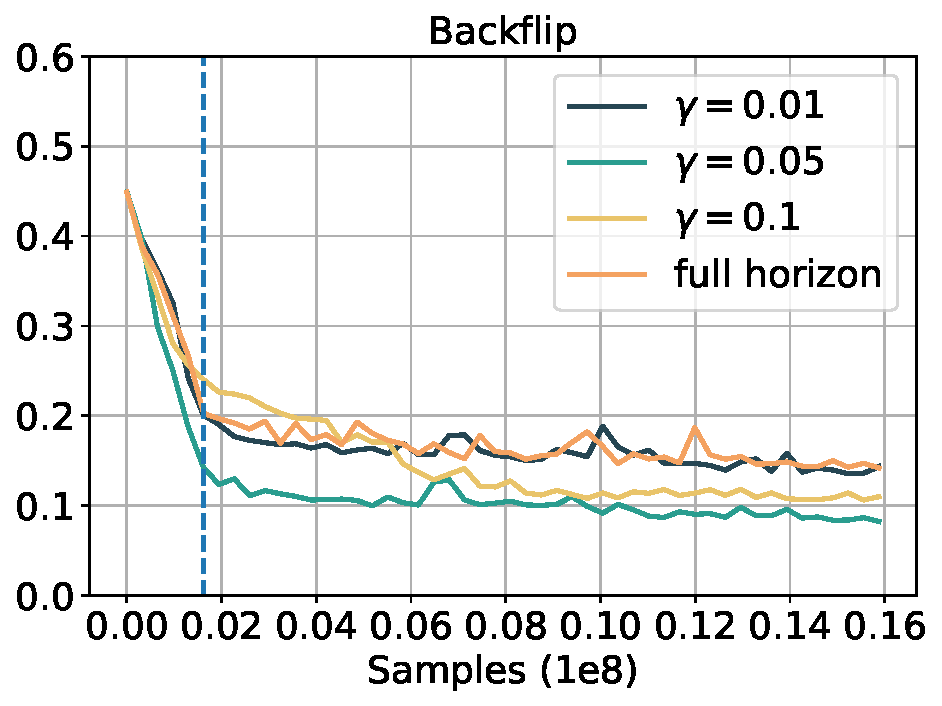
\includegraphics[width=0.3\textwidth]{figures/rand_backflip.pdf}&
    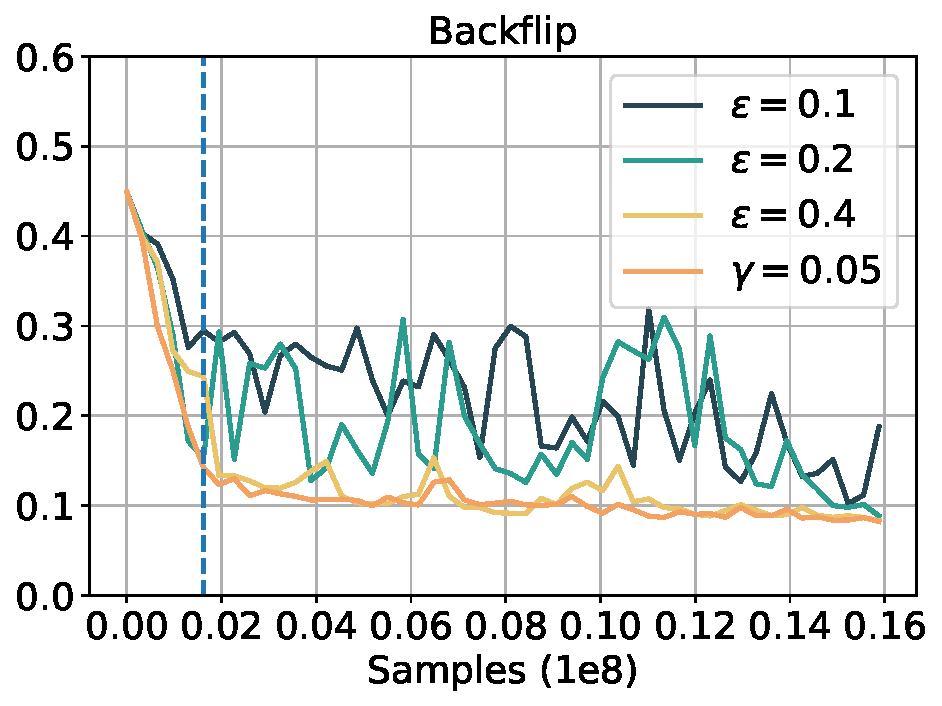
\includegraphics[width=0.3\textwidth]{figures/err_backflip.pdf}
    \\
    (a)
    &
    (c)
    &
    (e) 
    \\
    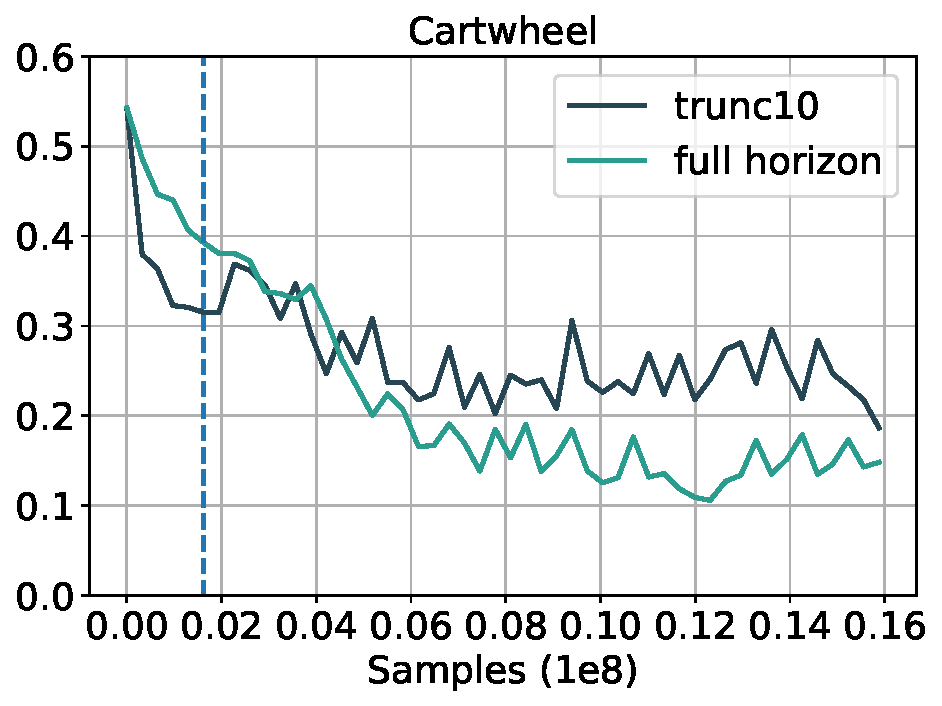
\includegraphics[width=0.3\textwidth]{figures/trunc_cartwheel.pdf}&
    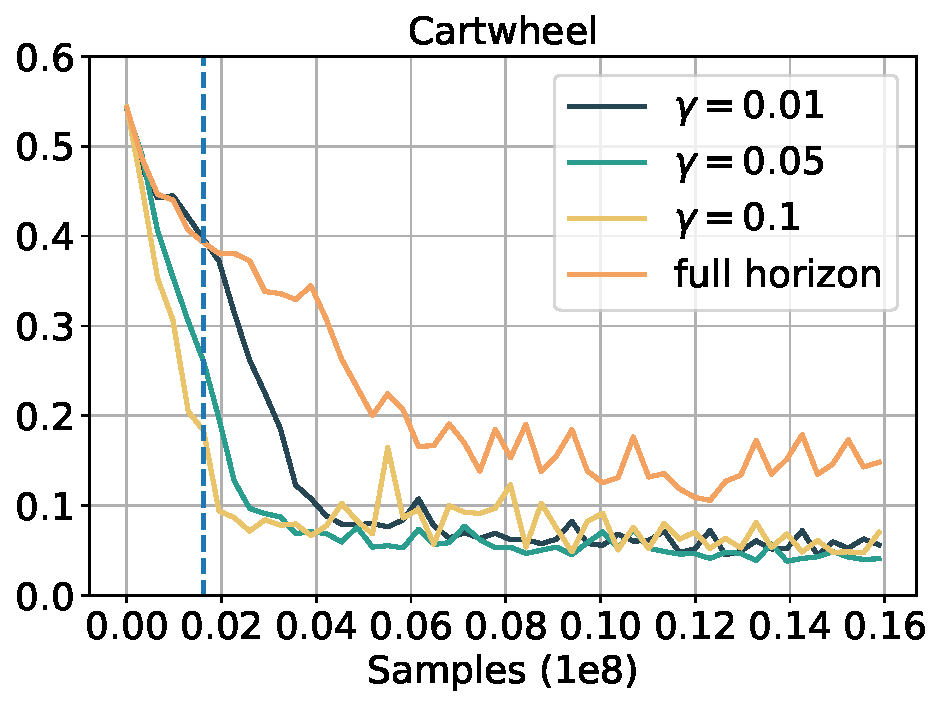
\includegraphics[width=0.3\textwidth]{figures/rand_cartwheel.pdf}&
    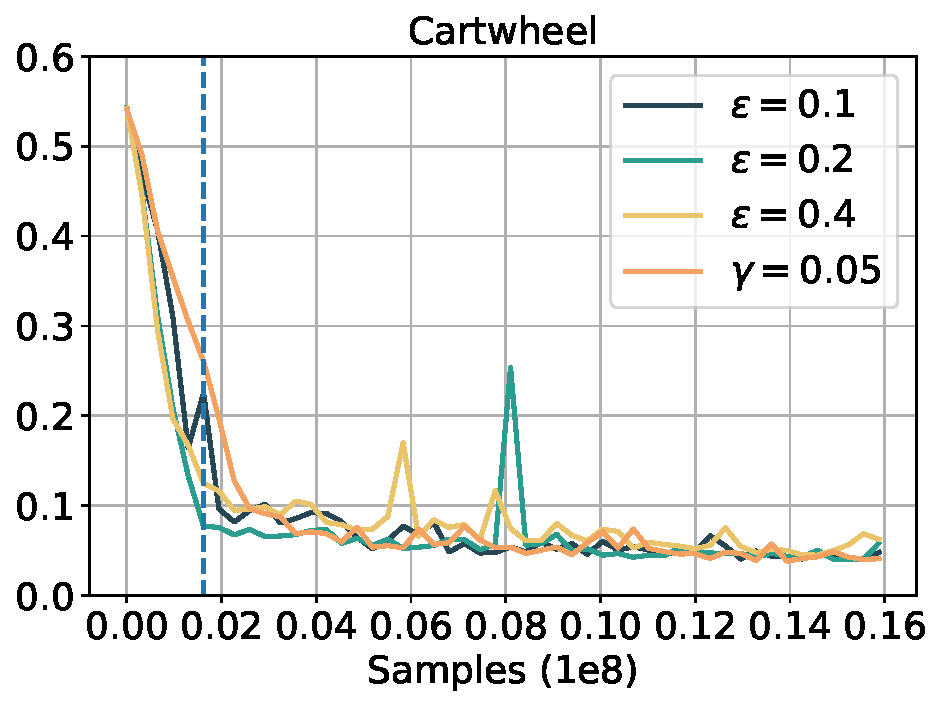
\includegraphics[width=0.3\textwidth]{figures/err_cartwheel.pdf}
    \\
    (b)
    &
    (d)
    &
    (f) 
    \end{tabular}
    \captionof{figure}{(a)-(b) Comparison between Full Horizon Gradient and truncation length of 10.
    (c)-(d)  Comparison between Demonstration Replay (Random) and Full Horizon Gradient.
    (e)-(f) Comparison between Demonstration Replay (Random) and Demonstration Replay (Threshold). The blue dotted line denotes 10 minutes in the corresponding wallclock time.}
    \vspace{-10pt}
    \label{tab:ablation}
\end{table}


To understand how demonstration replay affects the policy learning of DiffMimic, we compare three different variants of DiffMimic, namely, Demonstration Replay (Random) and Demonstration Replay (Threshold), and Full Horizon Gradient on \textit{Backflip} and \textit{Cartwheel}. Demonstration Replay (Random) randomly replaces a state in the rollout of the policy with the demonstration state at the same timestamp similar to the teacher forcing~\citep{williams1989learning}. Demonstration Replay (Threshold) inserts the demonstration state based on the pose error. If the pose error between the demonstration state and the simulated state exceeds a threshold $\epsilon$, the simulated state will be replaced by the demonstration state.
The Full Horizon Gradient variant backpropagates the gradient through the full horizon without any additional operation. We show the quantitative result in Fig.~\ref{tab:ablation}, and the qualitative result in Fig.~\ref{fig:vis_ablation}. 

\textbf{Demonstration replay helps stabilize policy learning and leads to better performance.} Compared with the Full Horizon Gradient without demonstration replay, the learning curve with demonstration replay is much smoother and finally converges to a lower pose error as shown in Fig.~\ref{tab:ablation} (c)-(d). We show in Fig.~\ref{fig:vis_ablation} (b), this vanilla version of DiffMimic can easily get stuck into a local minimum. Instead of learning to backflip, the policy learns to bend down and use arms to support itself instead of jumping up. The other two variants, by contrast, both learn to jump and backflip in mid-air successfully. 

\begin{wrapfigure}[19]{r}{0.38\columnwidth}
     \centering
     \vspace{-10pt}
     \centering
     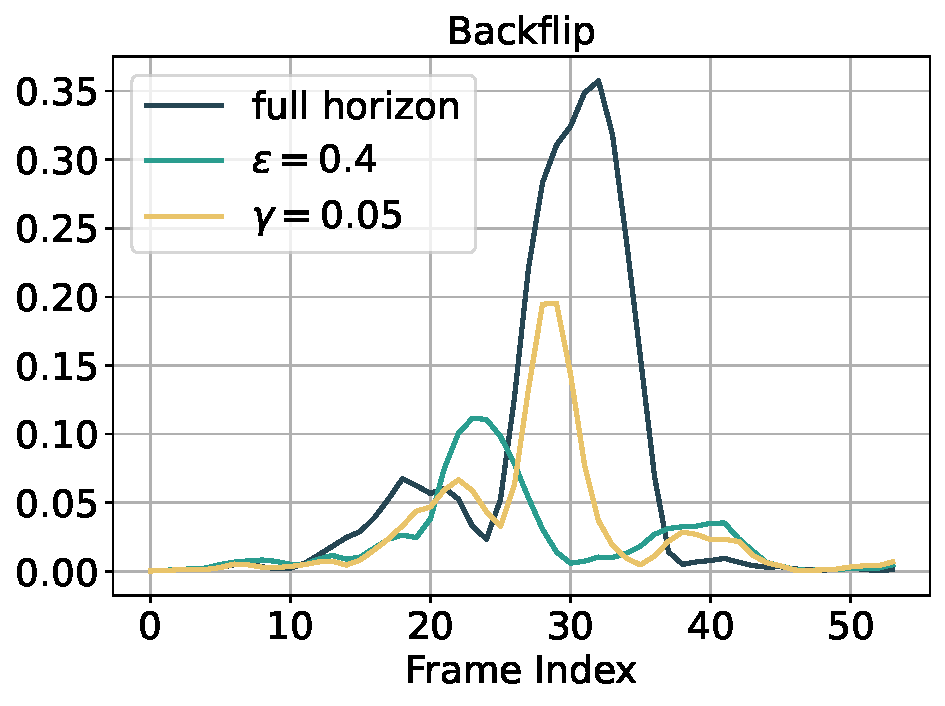
\includegraphics[width=0.38\textwidth]{figures/frame_backflip.pdf}
    \caption{L2 error per frame in the rollout of the final policy. Although Demonstration Replay (Random) reduces the overall pose error compared to full-horizon optimization, the per-frame loss remains large in certain time steps due to the lack of a constraint. Demonstration Replay (Threshold) alleviates the issue.}
    \label{fig:frame_loss}
\end{wrapfigure}
\textbf{Policy-aware demonstration replay leads to a more faithful recovery of demonstration.} 
We compare Demonstration Replay (Threshold) with Demonstration Replay (Random) in Fig.~\ref{tab:ablation} (e)-(f). Quantitatively, both variants yield similar results if the hyperparameter is properly tuned. However, the behavior of policies trained with these two strategies can be significantly different. In Fig.~\ref{fig:vis_ablation} (c) and (d), though both policies learn to backflip successfully, the policy trained with Demonstration Replay (Random) fails to recover the motion frame by frame. 
We show in Fig.~\ref{fig:frame_loss} the per-frame pose error. Even though the average error over the whole trajectory for both variants is similar, Demonstration Replay (Threshold) gives a lower maximum per-frame error, which indicates a faithful recovery of the demonstration. This implies that simply minimizing the pose error may not suffice to learn a policy that tracks the demonstration closely. Finer-grained guidance based on the current performance of the policy is required. 

















